Eingereicht:


\begin{minted}{text}
[t4, t3, t2, t1]
\end{minted}


t1 ist eine Transition des gegebenen Petrinetzes?\begin{quote}Yes.\end{quote}t2 ist eine Transition des gegebenen Petrinetzes?\begin{quote}Yes.\end{quote}t3 ist eine Transition des gegebenen Petrinetzes?\begin{quote}Yes.\end{quote}t4 ist eine Transition des gegebenen Petrinetzes?\begin{quote}Yes.\end{quote}Höchstens 8 Schritte angegeben?\begin{quote}Yes.\end{quote}Startmarkierung:

\begin{quote} [(s1,1),(s2,1),(s3,1),(s4,1)] \end{quote}Schritt 1

 Transition t4 

Zwischenmarkierung (nach Einziehen der Marken im Vorbereich)

\begin{quote} [(s1,0),(s2,1),(s3,1),(s4,0)] \end{quote}Endmarkierung (nach Austeilen der Marken im Nachbereich)

\begin{quote} [(s1,0),(s2,2),(s3,1),(s4,1)] \end{quote}

\begin{centering}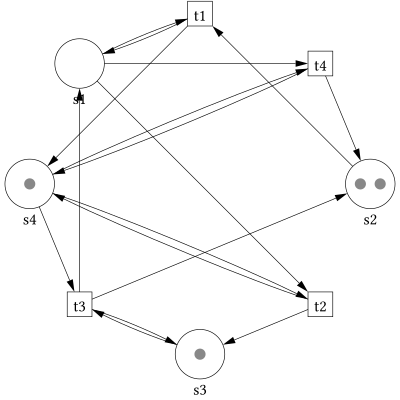
\includegraphics[min width=0.4\textwidth=0.6\textwidth,min height=0.4\textwidth=0.6\textwidth,keepaspectratio,max width=0.9\textwidth,max height=0.9\textwidth]{60/graph1petribff5ee5e2d580dc324d906b928cb642fdb23021043dc0552cc786557cea786f011013.pdf}\end{centering}

Schritt 2

 Transition t3 

Zwischenmarkierung (nach Einziehen der Marken im Vorbereich)

\begin{quote} [(s1,0),(s2,2),(s3,0),(s4,0)] \end{quote}Endmarkierung (nach Austeilen der Marken im Nachbereich)

\begin{quote} [(s1,1),(s2,3),(s3,1),(s4,0)] \end{quote}

\begin{centering}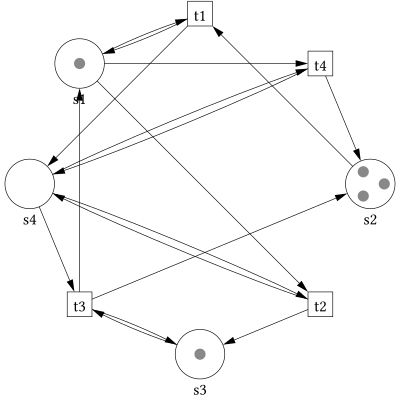
\includegraphics[min width=0.4\textwidth=0.6\textwidth,min height=0.4\textwidth=0.6\textwidth,keepaspectratio,max width=0.9\textwidth,max height=0.9\textwidth]{60/graph2petri07107e2f08eebcc8d629bc02f413fee5db0690a05d28ba7f397f45a479d1469d11013.pdf}\end{centering}

Schritt 3

 Transition t2 

Zwischenmarkierung (nach Einziehen der Marken im Vorbereich)

\begin{quote} [(s1,0),(s2,3),(s3,1),(s4,-1)] \end{quote}Enthält negative Markenanzahl (Transition war nicht aktiviert)!

Eine korrekte Lösung ist:
\begin{minted}{text}
[t3, t1, t3, t1, t1, t4, t1, t4]
\end{minted}


